\documentclass[a4paper]{article}

\usepackage{times}
\usepackage[ngerman]{babel}
\usepackage[T1]{fontenc}
\usepackage{amsmath}
\usepackage{amsfonts}
\usepackage{graphicx}
\usepackage{authblk}
\usepackage{fancyhdr}

\pagestyle{fancy}
\renewcommand{\headrulewidth}{0,6pt}
\fancyhead[L]{\leftmark}
\fancyhead[R]{\thepage}

\title{\Huge{Elektrik\\Lernzettel}}
\date{\today}
\author{\quad\\Baden, Julian\\Hagemann, Florian\\\quad\\Gymnasium Mellendorf\\ABI Jahr 2027}

\begin{document}

\maketitle
\thispagestyle{empty}
\newpage
\tableofcontents \thispagestyle{empty}
\newpage
\pagenumbering{arabic}

%________________________________________________________________________________________________

\section{Formelsammlung}
\subsection{Einheiten}

\begin{center}
    \begin{tabular}{ p{4cm} p{4cm} p{4cm} }
         Stromstärke            & $I$           & $A$                 \\[0,5cm]
         Ladung                 & $Q$ ($q$ für eine Probeladung)  & $C$ \\[0,5cm]
         Spannung               & $U$           & $V$                 \\[0,5cm]
         Wiederstand            & $R$           & $\Omega$            \\[0,5cm]
         el. Feldstärke         & $\vec{E}$     & $\dfrac{N}{C}$      \\[0,5cm]
         Kapazität              & $C$           & $F$                 \\[0,5cm]
         Flächenladungsdichte   & $\sigma$      & $\dfrac{C}{m^2}$    \\[1cm]
    \end{tabular}
\end{center}


\subsection{Formeln}
\paragraph{Stromstärke}
\large{$$I = \dfrac{Q}{t}$$}

\paragraph{Spannung}
\large{$$U = R \cdot I$$}





\subsubsection{Schaltungen von Widerständen}

\paragraph{Reihe}

\begin{center}
	\Large
		$I_{ges} = I_1 = I_2 = … = I_n$\\[0,5cm]
		$U_{ges} = U_1 + U_2 + … + U_n$\\[0,5cm]
		$R_{ges} = R_1 + R_2 + … + R_n$\\[1cm]
	\normalsize
\end{center}


\paragraph{Parallel}

\begin{center}
	\Large
		$I_{ges} = I_1 + I_2 + … + I_n$\\[0,5cm]
		$U_{ges} = U_1 = U_2 = … = U_n$\\[0,5cm]
		$\dfrac{1}{R_{ges}} = \dfrac{1}{R_1} + \dfrac{1}{R_2} + … + \dfrac{1}{R_n}$\\[1cm]
	\normalsize
\end{center}


\paragraph{Kirchhoff‘schen Gesetze (Bei Knotenpunkten)}

\begin{center}
    \Large 
        $\sum{I_{zufließend}} = \sum{I_{abfließend}}$\\[1cm]
    \normalsize
\end{center}



\subsubsection{Schaltungen von Kondensatoren}

\paragraph{Reihe}

\begin{center}
	\Large
		$Q_{ges} = Q_1 + Q_2 + … + Q_n$\\[0,5cm]
		$U_{ges} = U_1 + U_2 + … + U_n$\\[0,5cm]
		$\dfrac{1}{C_{ges}} = \dfrac{1}{C_1} + \dfrac{1}{C_2} + … + \dfrac{1}{C_n}$\\[1cm]
	\normalsize
\end{center}


\paragraph{Parallel}

\begin{center}
	\Large
		$Q_{ges} = Q_1 + Q_2 + … + Q_n$\\[0,5cm]
		$U_{ges} = U_1 = U_2 = … = U_n$\\[0,5cm]
		$C_{ges} = C_1 + C_2 + … + C_n$\\[1cm]
	\normalsize
\end{center}


\section{Elektrische Felder}

\subsection{Radialsymetrische Felder}
Bei Radialsymetrischen Feldern treten die Feldlinien radial (also sekrecht)
aus einer positiven Punktladung hervor.

\begin{figure} [h]
	\begin{center}
		\includegraphics[width=8cm]{Bilder/feldlinien_punktladung.png}
		\caption{Feldlinien von Punktladungen}
	\end{center}
\end{figure}

Feldlinien führen immer von + zu -.

\begin{figure} [h]
	\begin{center}
		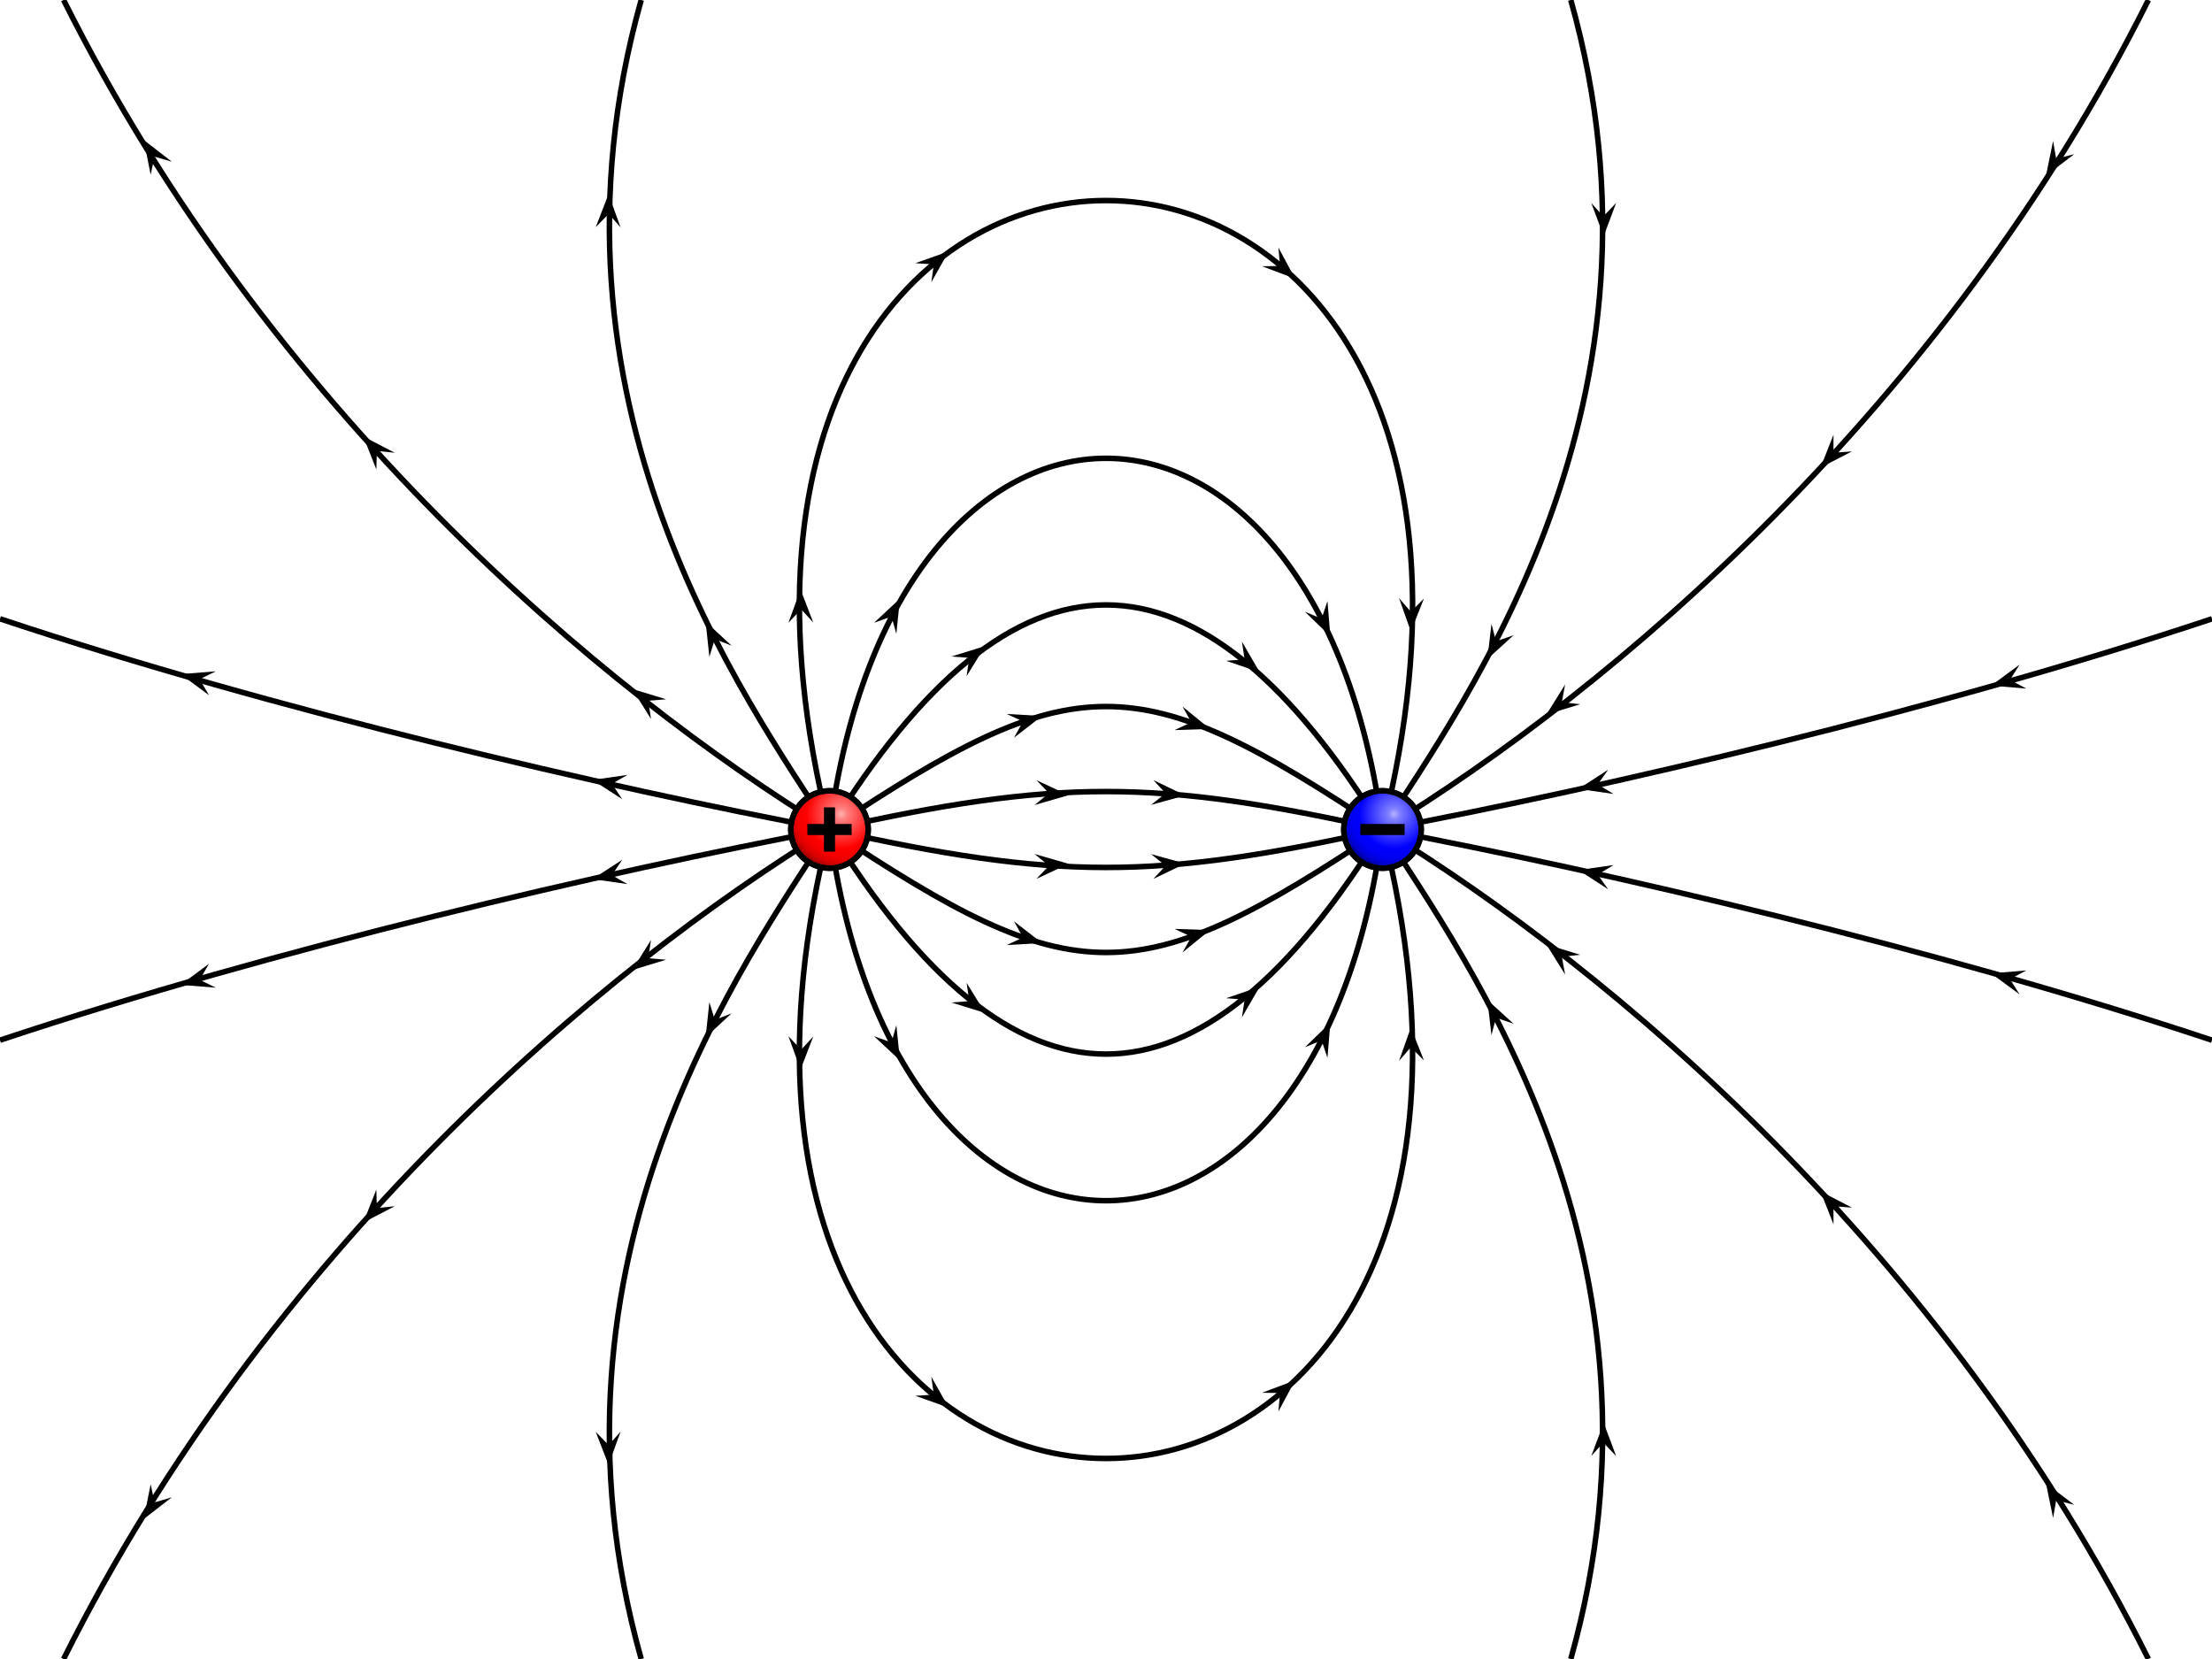
\includegraphics[width=8cm]{Bilder/field.png}
		\caption{Feldlinien von Punktladungen}
	\end{center}
\end{figure}



\subsubsection{Homologe Felder}
Zwischen zwei Kondensatorplatten herrscht ein homologes Feld. Zwischen ihnen verlaufen die feldlinien
direkt von + zu -. An den Randbereichen des Kondensators sind die Feldlinien gewölbt.

\begin{figure} [h]
	\begin{center}
		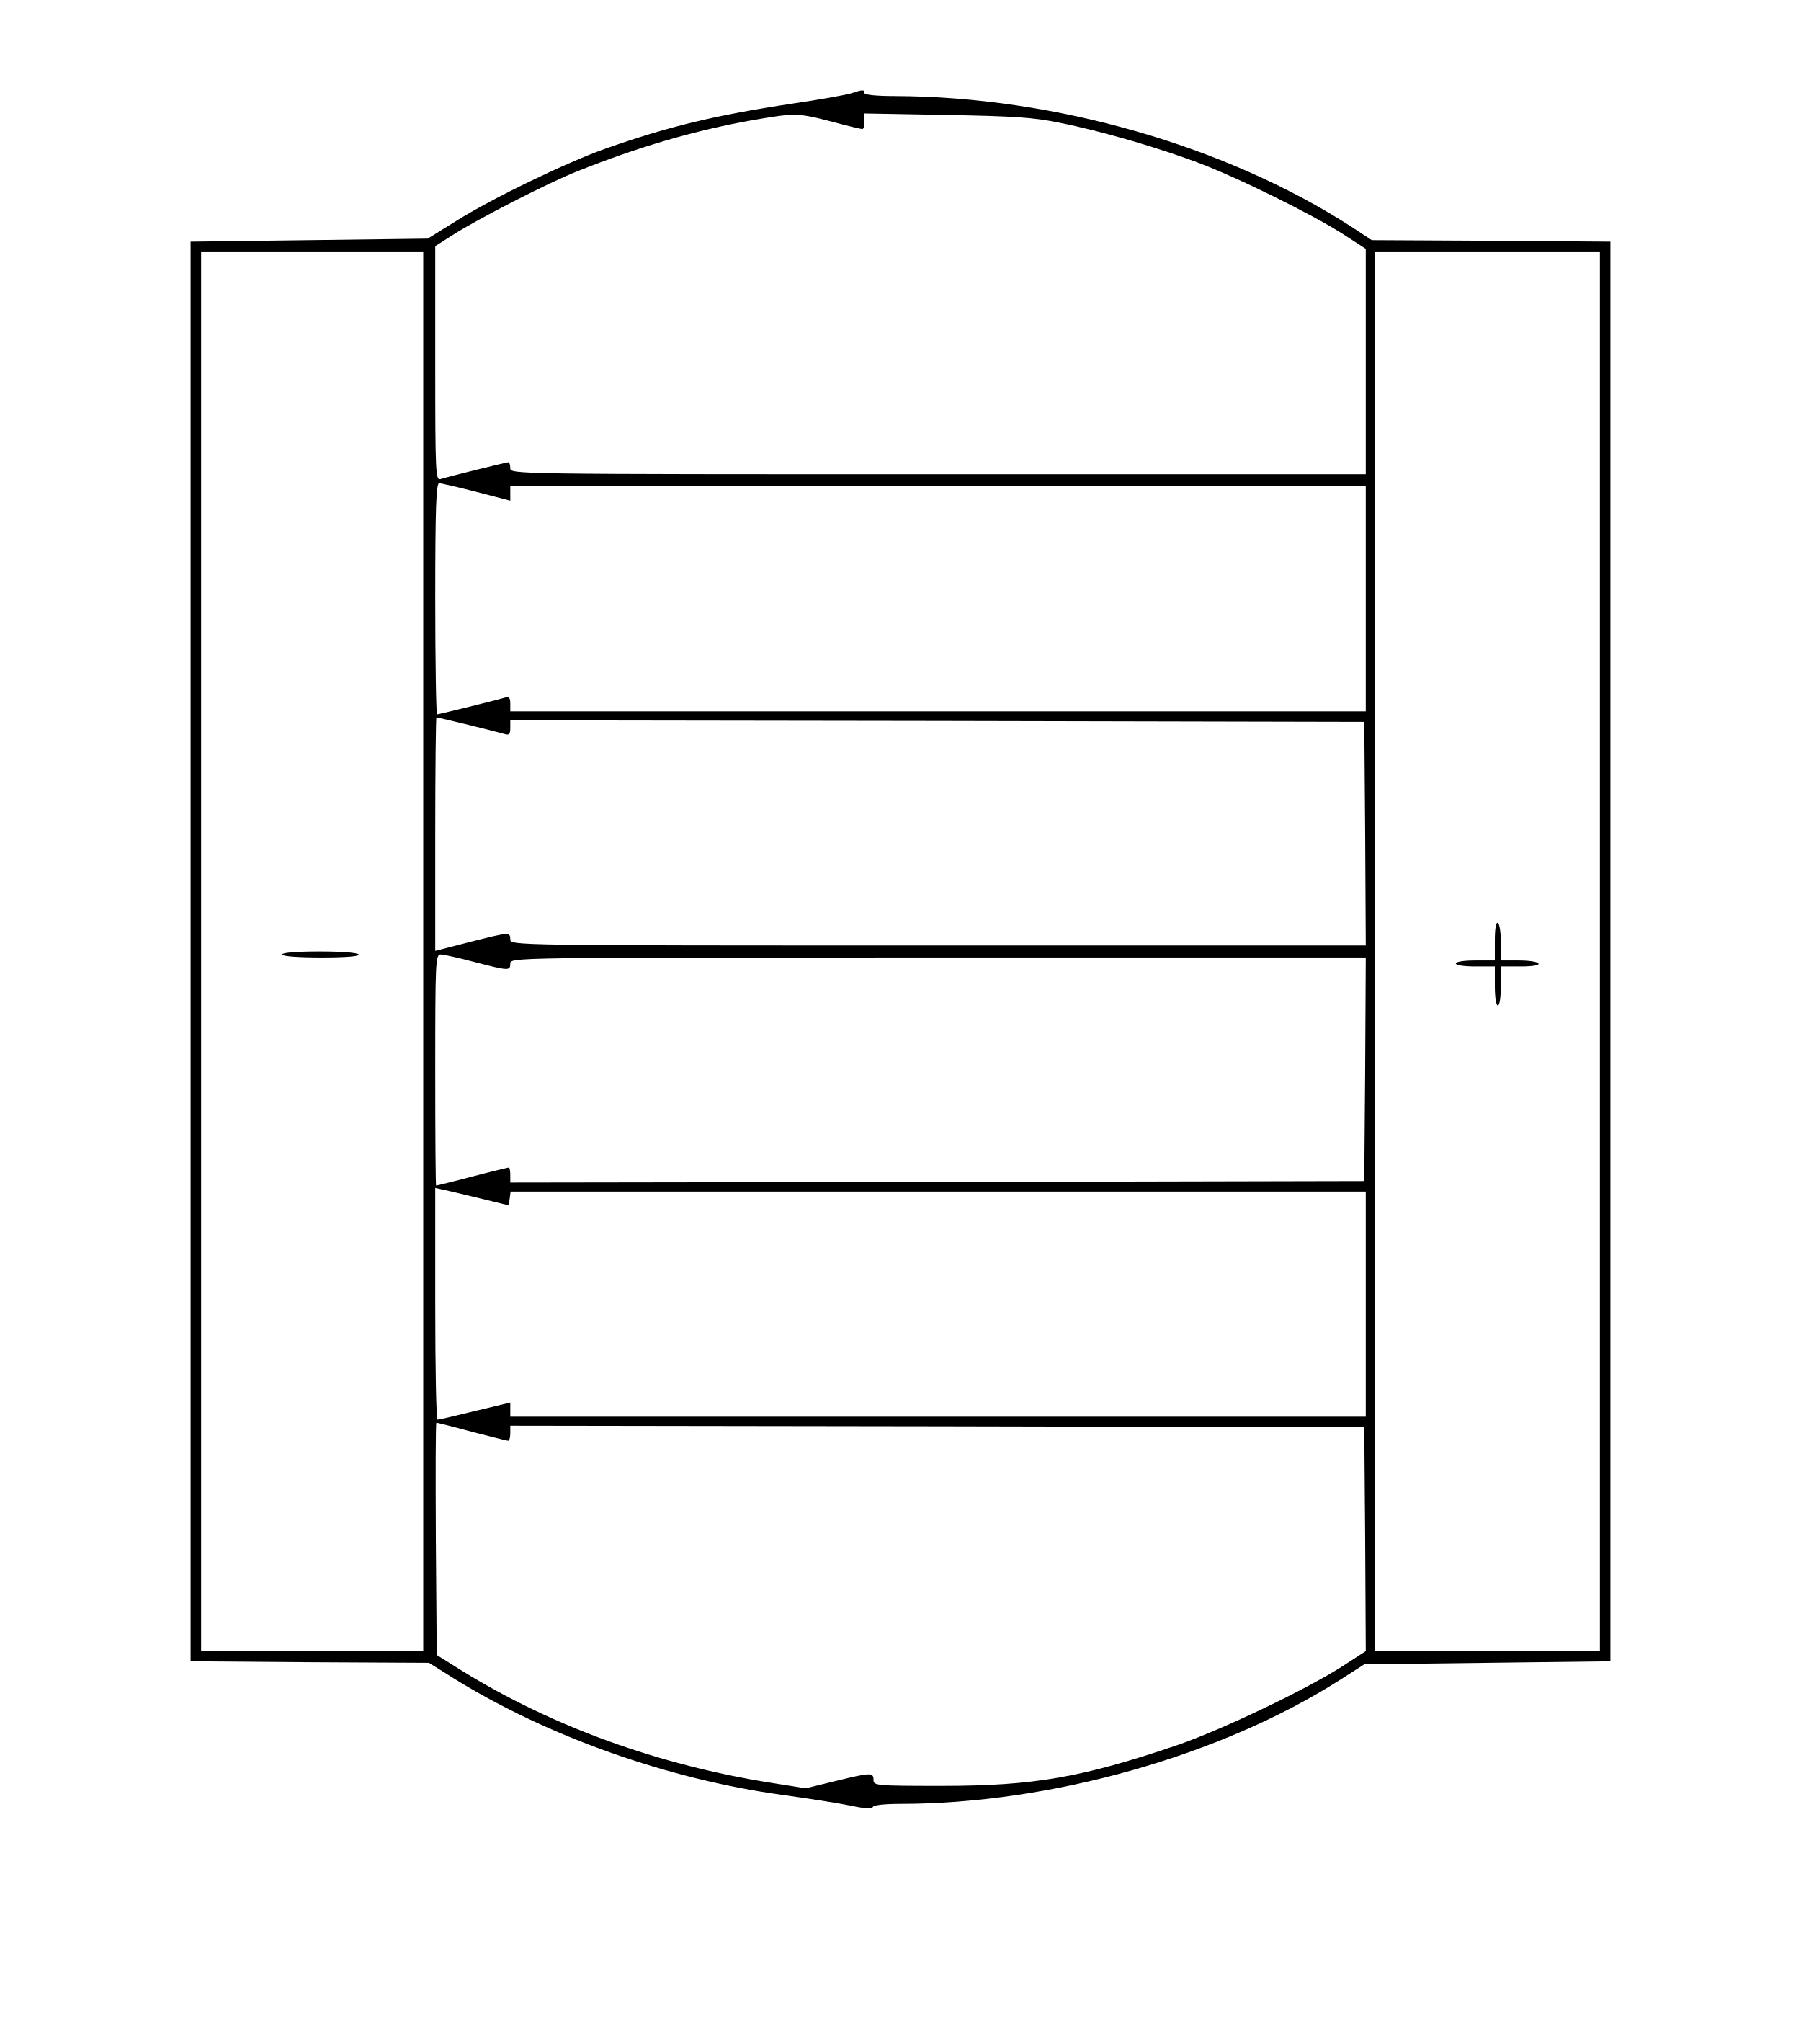
\includegraphics[width=8cm]{Bilder/homFeld.png}
		\caption{Feldlinien von homologen Feldern}
	\end{center}
\end{figure}



\subsection{Elektrische Feldstärke}
Die Elektrische Feldstärke ist proportional zur Kraft, die auf eine Probeladung wirkt und antiproportional
zur Ladung der Probeladung ($q$). Somit ergibt sich:

\Large$$\vec{E} = \dfrac{\vec{F}}{q}$$\normalsize\\




\subsubsection{Energie im homogenen elektrischen Feld}
Wenn sich eine Probeladung duch ein \textbf{homologes elektrisches Feld}, von einer Seite zur Anderen,
bewegt werden soll, wird eine Energie ($W$) benötigt. Diese berechnet sich durch:

\Large$$W = q \cdot \vec{E} \cdot d$$\normalsize\\

\begin{center}
	oder
\end{center}
\Large$$U = \dfrac{W}{q} = \vec{E} \cdot d$$\normalsize\\

Daraus ergibt sich für die \textbf{elektrische Feldstärke im homogenen elektrischen Feld}:

\Large$$\vec{E} = \dfrac{U}{d}$$\normalsize\\



\subsection{Flächenladungsdichte}







\end{document}